\section*{{Appendix:  Proofs}}





\stitle{Proof of Theorem~\ref{theo-ldrh-cised}}:
If $\dddot{\mathcal{T}}_s$ can be represented by line segment $\overline{P_sP_{s+k}}$ by algorithm \ldrh, then we have $|P_{s+i}P'_{s+i}| < \epsilon/2$ for each $i \in (0, k)$, where $P'_{s+i}$ is the expected position (synchronized point) of $P_{s+i}$ \wrt the initial velocity $\vv{v}$ of \ldrh.
From the view of the ``x-y-t" 3D space, $\vv{v}$ must be in the common intersection of  $\bigsqcap_{i=1}^{k}$\cone{(P_s, P_{s+i}, \epsilon/2)}, in other words, we have $\bigsqcap_{i=1}^{k}$\cone{(P_s, P_{s+i}, \epsilon/2)} $\ne \{P_s\}$, meaning this sub-trajectory can be represented by approaches based on the spatio-temporal cones.
\eop

\stitle{Proof of Theorem~\ref{theo-full-cone}}:
Let $P'_{s+i}$ be the intersection point of line segment $\overline{P_sP_{s+k}}$ and plane $t = P_{s+i}.t,~i\in (0,k)$, indeed, $P_{s+i}$ is the synchronized point of $P_{s+i}$ \wrt line segment $\overline{P_sP_{s+k}}$. 
Because $\overline{P_sP_{s+k}}$ passes through $\bigsqcap_{i=1}^{k-1}$\cone{(P_s, P_{s+i}, \epsilon)} - \{$P_s$\}, $P'_{s+i}$ must be inside of the synchronous circle of $P_{s+i}$ on the plane. Thus we have $|P_{s+i}P'_{s+i}|<\epsilon$, \ie $sed(P_{s+i}, \overline{P_sP_{s+k}})|<\epsilon$.
\eop

\stitle{Proof of Theorem~\ref{theo-cone-vs}}:
(1) If $\bigsqcap_{i=1}^{k}$\cone{(P_s, P_{s+i}, \epsilon/2)} $\ne \{P_s\}$, then $sed(P_{s+i}, P_sP_{s+k}) <\epsilon$ for each $i \in [1,k]$. 
The intersection point  $P'_{s+i}$ of line segment $P_s P_{s+k}$ and plane $t = P_{s+i}.t$ is the synchronized point of $P_{s+i}$ \wrt $P_s P_{s+k}$, such that $|P_{s+i}P'_{s+i]}| < \epsilon$. Hence for each $i \in [1,k]$, $P'_{s+i}$ falls in the synchronous circle of $P_{s+i}$ on the plane, meaning $\overline{P_sP_{s+k}}$ passes through the common intersection of the preview cones $\bigsqcap_{i=1}^{k-1}$\cone{(P_s, P_{s+i}, \epsilon)}-$\{P_s\}$.
%
(2) If line segment $\overline{P_sP_{s+k}}$ passes through the common intersection $\bigsqcap_{i=1}^{k-1}$\cone{(P_s, P_{s+i}, \epsilon)} - \{$P_s$\}, then, suppose there is $i$ and $j$ ($i<j<k$) such that $P^{s+j}_{s+i}$ and $P^{s+k}_{s+i}$ are the intersection points of $\overline{P_sP_{s+j}}$ and $\overline{P_sP_{s+k}}$ with the plane $t = P_{s+i}.t$, respectively, we have $0 \le |P_{s+i}P^{s+k}_{s+i}|<\epsilon$ and $0 \le |P^{s+j}_{s+i}P^{s+k}_{s+i}|<\epsilon$, meaning $0 \le |P_{s+i}P^{s+j}_{s+i}|<2\epsilon$, \ie~$|P_{s+i}P^{s+j}_{s+i}|$ is not necessarily less than $\epsilon$. 
%
If it is greater than $\epsilon$, then the intersection of \cone{(P_s,P_{s+i},\epsilon/2)} and \cone{(P_s,P_{s+j},\epsilon/2)} is $\{P_s\}$, and $\bigsqcap_{i=1}^{k}$\cone{(P_s, P_{s+i}, \epsilon/2)} is also $\{P_s\}$.
%
Combine (1) and (2) we have the conclusion.
\eop

\stitle{Proof of Theorem~\ref{theo-half-sector}}:
Trajectory tracking is the combination of trajectory simplification and position tracking.
%
(1) Trajectory simplification: It can be simplified in strip-like areas as illustrated in Section \ref{sec:track_cone_sector};
%
(2) Position tracking: If it can be represented by a line segment by the intersection of sectors, then there is sure a $\vv{v}$ living in the common intersection of sectors, \eg $\vv{v}$ on $P_sP_{s+i}$, such that it is applicable to track the position in strip areas.
%
Combine (1) and (2), we have the conclusion.
\eop


\stitle{{Proof of Theorem~\ref{theo-full-sector}}}:
First, let $|P_sP_{s+k}| = \sqrt{l_m^2 - \epsilon^2}$. We draw an arc $\widehat{BD}$ taking $P_s$ as its center and $l_m$ as its radius, and two lines $\overline{AB}$ and $\overline{CD}$ paralleling and having a distance of $\epsilon$ to $\overline{P_sP_{s+k}}$, as shown in Figure \ref{fig:sectorinter}.
Because line segment $\overline{P_sP_{s+k}}$ passes through $\bigsqcap_{i=1}^{k-1}$\sector{(P_s, P_{s+j}, \epsilon)}- $\{P_s\}$ and $l_{m} = max\{|P_sP_{s+i}|\}$ for each $i \in (0, k)$, point $P_{s+i}$ must live in the area between lines $\overline{AB}$ and $\overline{CD}$, and in the inner side of arc $\widehat{BD}$.
(1) If $P_{s+i}$ is between $\overline{BD}$ and $\widehat{BD}$, then $ped(P_{s+i}, \overline{P_sP_{s+k}}) = |{P_{s+i}P_{s+k}}| < |{BP_{s+k}}| = \epsilon$; 
(2) If $P_{s+i}$ is in the left side of $\overline{BD}$, then  $ped(P_{s+i}, \overline{P_sP_{s+k}})$ is the perpendicular Euclidean distance from $P_{s+i}$ to the line segment $\overline{P_sP_{s+k}}$ that is also less than $\epsilon$. Combining (1) and (2) we have $ped(P_{s+i}, \overline{P_sP_{s+k}})< \epsilon$ for $|P_sP_{s+k}| = \sqrt{l_m^2 - \epsilon^2}$.
Next, it is easy to find that if $|P_sP_{s+k}| > \sqrt{l_m^2 - \epsilon^2}$ then the conclusion remains the same.
%then for each point $P_{s+i}$, $i\in (0,k)$, it has a Euclidean distance $d_i$ less than $\epsilon$ to the line that $\overline{P_sP_{s+k}}$ lives on. We also know that $\overline{P_sP_{s+k}}$ is not shorter than any other line segment, thus, the distance $d_i$ is indeed the \ped of $P_{s+i}$ to the line segment $\overline{P_sP_{s+k}}$. That is, $ped(P_{s+i}, P_sP_{s+k}) <\epsilon$ for each $i\in (0,k)$.
\eop

\begin{figure}[tb!]
	\centering
	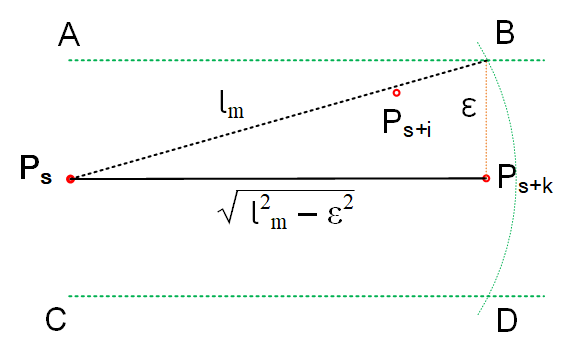
\includegraphics[scale=1.0]{figures/Fig-SectorInter.png}
	\vspace{-2ex}
	\caption{\small The intersection of full-$\epsilon$ sectors.  }
	\vspace{-1ex}
	\label{fig:sectorinter}
\end{figure}

\eat{%%%%%%%%%%%%%%%%%%%%%%%%%%%%%%%%%%
\stitle{\textcolor{red}{Proof of Theorem~\ref{theo-full-sector}}}:
If line segment $\overline{P_sP_{s+k}}$ passes through $\bigsqcap_{i=1}^{k-1}$\sector{(P_s, P_{s+j}, \epsilon)}- $\{P_s\}$, \ie it lives in all the preview sectors, then for each point $P_{s+i}$, $i\in (0,k)$, it has a Euclidean distance $d_i$ less than $\epsilon$ to the line that $\overline{P_sP_{s+k}}$ lives on. We also know that $\overline{P_sP_{s+k}}$ is not shorter than any other line segment, thus, the distance $d_i$ is indeed the \ped of $P_{s+i}$ to the line segment $\overline{P_sP_{s+k}}$. That is, $ped(P_{s+i}, P_sP_{s+k}) <\epsilon$ for each $i\in (0,k)$.
\eop

\stitle{Proof of Theorem~\ref{theo-sector-vs}}:
(1) If $\bigsqcap_{i=1}^{k}$\sector{(P_s, P_{s+i}, \epsilon/2)} $\ne \{P_s\}$, then $\overline{P_sP_{s+k}}$ lives in the common intersection of the preview half-$\epsilon$ sectors. 
Hence, it is sure living in the common intersection of the preview full-$\epsilon$ sectors, \ie it passes through $\bigsqcap_{i=1}^{k-1}$\sector{(P_s, P_{s+i}, \epsilon)} $- \{P_s\}$.
%
(2) If line segment $\overline{P_sP_{s+k}}$ passes through the common intersection $\bigsqcap_{i=1}^{k-1}$\sector{(P_s, P_{s+i}, \epsilon)} - \{$P_s$\}, then, given $i$ and $j$ ($i<j<k$), it is possible that $ped(P_{s+i}, \overline{P_sP_{s+k}})> \epsilon/2$ and $ped(P_{s+j}, \overline{P_sP_{s+k}})> \epsilon/2$ , meaning the intersection of \sector{(P_s,P_{s+i},\epsilon/2)} and \sector{(P_s,P_{s+j},\epsilon/2)} is $\{P_s\}$, and thus, $\bigsqcap_{i=1}^{k}$\sector{(P_s, P_{s+i}, \epsilon/2)} is also $\{P_s\}$.
%
Combine (1) and (2) we have the conclusion.
\eop
}%%%%%%%%%%%%%%%%%%%%%%%%%%%%%%%%%%%%%

\stitle{Proof of Theorem~\ref{theo-binary}}:
Given a sub-trajectory $[P_s,...,P_{s+k}]$ and two error bounds $\epsilon_{sed}$ and $\epsilon_{ped}$ satisfying $\epsilon_{sed} > \epsilon_{ped}$, from Theorems~\ref{theo-ldrh-cised} and \ref{theo-half-sector}, we know this sub-trajectory can be tracked in a circular and a strip areas, respectively.  
%
(1) Trajectory simplification: Let $\overline{P_sP_{s+i}}, i\in (0,k],$ be the line segment representing sub-trajectory $[P_s,...,P_{s+i}]$, because $\epsilon_{sed} > \epsilon_{ped}$, these areas indeed form a rectangle-like area, \ie this sub-trajectory can be simplified in rectangle-like areas by combining sectors and spatio-temporal cones.
%
(2) Position tracking: If the sub-trajectory $[P_s,...,P_{s+i}]$ can be represented by line segment $\overline{P_sP_{s+i}}$ by the intersections of sectors and cones, then there is sure a velocity $\vv{v}$ living in the common intersections of cones and sectors, such that it is applicable to track the position of the moving object in a rectangular-like area \wrt the $P_s$ and $\vec{v}$. 
Combine (1) and (2) we have the conclusion.
\eop


